%\documentclass{article}
\documentclass{article}
\usepackage{tikz}
\usepackage{tikz-dependency}
\usepackage{multirow}
\usepackage{caption} 
\captionsetup[table]{skip=10pt}
\usepackage{array}
\newcolumntype{C}[1]{>{\centering\let\newline\\\arraybackslash\hspace{0pt}}m{#1}}
\usepackage[T1]{fontenc}




\begin{document}

\begin{table}[ht] 
   \begin{tabular}{c | l }
%      catena &  type & \hspace{1cm}HI \hspace{2.8cm}Mixed & HF \hspace{1cm} \\
 \hline
 hierarchical  catena & \parbox[c]{22em}{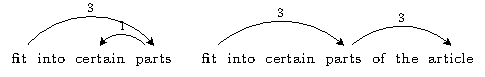
\includegraphics[width=8cm, height=1.8cm]{hierarchical/hier-cat-ex.pdf}} \\
  \hline
parallel  catena & \parbox[c]{8em}{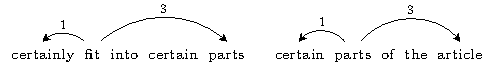
\includegraphics[width=8cm, height=1.8cm]{parallel/para-cat-ex.pdf}} \\
    \hline
  \end{tabular}
\end{table}

\end{document}